% Document Setup
\documentclass[12pt,a4paper,twoside]{book}

\usepackage[utf8]{inputenc}
\usepackage[a4paper,inner=3.5cm,outer=2.5cm]{geometry}
\usepackage[titletoc,title,toc,page]{appendix}
\usepackage{verbatim}
\usepackage{placeins}
\usepackage{listings}
\usepackage{xurl}
\usepackage[hidelinks]{hyperref}
\usepackage[english]{babel}
\usepackage{tikz}
\usepackage{parskip}
\usepackage{graphicx}
\usepackage{blindtext}
\usepackage{chngcntr}
\counterwithin{table}{chapter}

\usepackage{newlfont}
\usepackage{fancyhdr}
\usepackage{indentfirst}
\usepackage[utf8]{inputenc}
\usepackage{float}
\usepackage[capitalize,noabbrev]{cleveref}
\usepackage{soul}
\usepackage[font=footnotesize,labelfont=bf]{caption}

\usepackage{multirow}
\usepackage{hyphenat}
\hyphenation{mate-mati-ca recu-perare}

\usepackage{lscape} 

\usepackage{pdfpages}
% -----------------------------------------------------------------------------
% Bibliography Setup
\usepackage{natbib}
\bibliographystyle{alpha}
\setcitestyle{super,open={[},close={]}}

\newcommand{\rom}[1]{\uppercase\expandafter{\romannumeral #1\relax}}

% -----------------------------------------------------------------------------
% Begin Document
\begin{document}
% Per spostare i vari elementi più su o più giù gioca con i valori di vspace che ci sono tra uno e l'altro
\pagestyle{empty}
\newgeometry{
    left=20mm,
    right=20mm,
    top=20mm,
    bottom=20mm
}

% -----------------------------------------------------------------------------
% Title Page
\begin{titlepage}

\begin{center}

\includegraphics[width=6.5cm,height=4.7cm]{img/logo/marchio-di-ateneo.png}

\vspace{10mm}

{\Large{\bf{DOTTORATO DI RICERCA IN
MECCANICA E SCIENZE AVANZATE DELL'INGEGNERIA}}}

\vspace{15mm}

{\huge{\bf Open Methods for Digital Conservation of Musical Instruments }}\\
\vspace{3mm}

\end{center}

\vspace{10mm}

\begin{minipage}[t]{0.40\textwidth}
{\Large{\bf Supervisore: \\ Dr. Michele Ducceschi}}
\vspace{3mm}
{\Large{\bf Co-supervisore: \\ Dr. Federico Fontana }}
\end{minipage}
\hfill
\begin{minipage}[t]{0.40\textwidth}\raggedleft
{\Large{\bf Presentata da: \\ Matthew Hamilton}}
\end{minipage}


\vspace{8cm}

\begin{center}
\rule[0.0cm]{\linewidth}{0.1mm}\\
{\large{\bf Esame finale anno 2026 \\}}
\end{center}

\end{titlepage}

% -----------------------------------------------------------------------------
% Abstract Page
\newpage~\newpage
\pagenumbering{gobble}
%%%%%%%%%%%%%%%%%%%%%%%%%%%%%%%%%%%%%%%%%%%%%%%%%%%%%%%%%%
% Acoustics and Music Technology Final Project Latex Template
%
% ABSTRACT PAGE
%
% TOTAL EDITS REQUIRED: 1
%%%%%%%%%%%%%%%%%%%%%%%%%%%%%%%%%%%%%%%%%%%%%%%%%%%%%%%%%%


\begin{abstract}


%%%%%%%%%%%% EDIT %%%%%%%%%%%%
I made a plan, I carried it out. The results are amazing. Please give me a job. And buy me a beer. The end.
%%%%%%%%%%%% EDIT %%%%%%%%%%%%


\end{abstract}
\topmargin=-1cm
% -----------------------------------------------------------------------------
% Dedication Page

\newpage

\topmargin=6.5cm
\begin{flushright}
\emph{
\LARGE{La dedica}\\\vspace{2mm}
\LARGE{anche quella se vuoi}\\\vspace{3mm} 
\LARGE{su più righe} 
}
\end{flushright}

% -----------------------------------------------------------------------------
% TOCs
\tableofcontents
\thispagestyle{empty}
\listoftables
\thispagestyle{empty}
\listoffigures
\thispagestyle{empty}
\newpage~\newpage

% -----------------------------------------------------------------------------
% Chapters

% \pagenumbering{arabic}
% \setcounter{chapter}{-1}
% \raggedbottom
% \chapter{INTRODUZIONE} \label{chap:intro}
% \pagestyle{plain}
% \setcounter{page}{1}

\chapter{Introduction}\label{chapter-1}
\section{Problem of Digital Conservation of Musical Instruments}
\section{Open Science}
\subsection{F.A.I.R.}
\subsection{Open Science for Teaching}
\subsection{Sustainable Software Engineering}
\section{Digital Conservation}
\subsection{Musical Instruments and Digital Cultural Heritage}
\section{Thesis Structure}



%%%%%%%%%%%%%%%%%%%%%%%%%%%%%%%%%%%%%%%%%%%%%%%%%%%%%%%%%%
% Acoustics and Music Technology Final Project Latex Template
%
% CHAPTER 2 PAGE
%
% TOTAL EDITS REQUIRED: 1
%
% NOTE: NO NEED TO INCLUDE ANY FURTHER PREAMBLE IN THIS FILE
%%%%%%%%%%%%%%%%%%%%%%%%%%%%%%%%%%%%%%%%%%%%%%%%%%%%%%%%%%



\chapter{Measurement: Open Laser Vibrometry}\label{measurement-open-laser-vibrometry}

\section{The Problem}\label{the-problem-1}

\subsection{Vibrometry Theory}\label{vibrometry-theory}

\subsection{Measuring Plates}\label{measuring-plates}

\section{The Solution}\label{the-solution}

\subsection{Designing a vibrometer}\label{designing-a-vibrometer}

\subsection{Design Decisions}\label{design-decisions}

\subsection{Limitations}\label{limitations}

\section{Application}\label{application}

%%%%%%%%%%%% EDIT %%%%%%%%%%%%
\chapter{Finite Difference Time Domain}
\label{chapter2}
%%%REVISE THIS SECTION
The finite-difference time-domain method is a technique which is considered to be one of the most intuitive and simplest ways to approximate a continuous variable function \textit{u(t)} (Bilbao/Schneider) by time series. To approximate this continuous function we say that $u(t_{n})=u(nk)$ for integer $n$, where \textit{k} is considered to be the time step between each value in the time series.\\
In regard to musical applications, these technique yields very interesting and accurate results. This is due to the fact that, as for most audio applications the step time is relatively small. Considering that in audio, the sampling rate is standarized to normally about 44100 Hz, we can see how this time step $k=1/Fs$, will be small enough so that information is preserved with a good degree of accuracy. 

\section{Difference operators}
\label{chapter2:sec1}
In order to produce an approximation to a continuous function through a time series, it is necessary to define a series of operators that are applied to the the approximation. In this case, the operators that are necessary to simulate the function at a particular time will involve different time steps of the approximating series. Therefore for a time series ${u}^{n}$ where $n$ represents the $n^{th}$ time step, it is necessary to introduce the following 
\begin{equation*}
	e_{t+}u^{n} = u^{n+1}  \ \ \ \ \ \  e_{t-}u^{n} = u^{n-1}    \ \ \ \ \       $ e_{t+}e_{t-} = 1
\end{equation*}
These operators are defined as forward and backwards shifts respectively. Thanks to these operators, it is possible to approximate a wide variety of continuous operators, although for the purposes of this paper they will be limited to approximate first and second derivatives.
To produce an approximation to the first derivative operator, it is possible to use different combinations of the backward and forward shifts as follows,
\begin{equation}
	\begin{aligned}
	\delta_{t+} \overset{\Delta}{=} \frac{1}{k} (e_{t+} -1) \cong \frac{d}{dt}
	\end{aligned}
\end{equation}
\begin{equation}
	\begin{aligned}
	\delta_{t-} \overset{\Delta}{=} \frac{1}{k} (1 - e_{t-}) \cong \frac{d}{dt}	
	\end{aligned}
\end{equation}
\begin{equation}
	\begin{aligned}
	\delta_{t\cdot} \overset{\Delta}{=}  \frac{1}{2k} (e_{t+} -e_{t-}) \cong \frac{d}{dt}
	\end{aligned}
\end{equation}
These operators are defined as forward, backward, and centered difference operator respectively.\\ 
It is possible to extend this techinique to higher order derivatives, like for example second order derivatives. To do so, we will require the product of two of the previous difference operators. Hence, the second order difference operator \textit{$\delta_{tt}$} is defined by
\begin{equation}
\label{eqn:ddiff}
	\begin{aligned}
	\delta_{tt} \overset{\Delta}{=} \delta_{t+}\delta_{t-}=\frac{1}{k^2}(e_{t+}-2+e_{t-})\cong\frac{d^2}{dt^2}
	\end{aligned}
\end{equation}  
The reader at this point might have already realized the possibility of combining difference operators to for example approximate second order partial derivatives, this approximation consists on the product of two difference operators acting on different variables. As an example, we will consider the approximation to the double partial derivative $\frac{\partial^{2}}{\partial x \partial y}$,
\begin{equation}
	\begin{aligned}
	\delta_{x+}\delta_{y-}  \overset{\Delta}{=} \frac{1}{k^2} (e_{x+} -1) (1-e_{y-} )=\\
		=\frac{1}{k^2}(e_{x+}-e_{x+}e_{y-}-1+e_{y-}) \cong  \frac{\partial^2}{\partial x \partial y}
	\end{aligned}
\end{equation}


%%%%%%%%%%%% EDIT %%%%%%%%%%%%
\chapter{Analysis: Magpie}\label{chapter-3}

\section{The Problem}\label{the-problem-2}

\subsection{Plate Theory}\label{plate-theory}

\subsection{Boundary Conditions}\label{boundary-conditions}

\section{The Solution}\label{the-solution-1}

\subsection{Implementation}\label{implementation}

\subsubsection{Discretising}\label{discretising}
\subsubsection{Design}\label{design}

\section{Application}\label{application-1}

\chapter{Interaction: A MIDI Harpsichord Interface with Tactile Response}\label{chapter-4}

\section{The Problem}\label{the-problem-3}

\subsection{Musical Haptics}\label{musical-haptics}

\subsection{Harpsichord Haptics}\label{harpsichord-haptics}

\subsubsection{Player Perception}\label{musical-haptics}
\subsubsection{Haptics and Pedagogy}\label{musical-haptics}

\section{Creation of Hardware Interface}\label{the-solution-2}
\subsection{Design Principles}\label{design}
\subsection{Materials and Construction}
\subsubsection{3-Key Model}
\subsubsection{Full Model}
\subsubsection{Problems of Scale}

\subsection{Project Deployment}
\subsubsection{Experiments in Jack Tracking}\label{experiments-in-jack-tracking}
\subsubsection{Refinement of QRE1113}\label{refinement-of-qre1113}


\section{Electronics Design}\label{hardware-design}
\subsection{First Prototype}
\subsubsection{Sensor Board}\label{sensor-board}
\subsubsection{Controller Board}\label{controller-board}
\subsubsection{Bracket Design}\label{controller-board}
\subsection{Second Prototype}
- introduction of FSR data
\subsubsection{Sensor Board}\label{sensor-board}
\subsubsection{Controller Board}\label{controller-board}
\subsubsection{Bracket Design}\label{controller-board}

\section{Firmware Design}\label{hardware-design}
\subsection{Interfacing with digital instrument}\label{interfacing-with-digital-instrument}
\subsection{Custom MIDI standard}\label{custom-midi-standard}

\section{Application}\label{application-2}
\subsection{Exhbition}\label{interfacing-with-digital-instrument}


\section{Introduction}\label{introduction}

Technological advances have transformed how museums document, present and interpret their collections. Immersive experiences are realised through tools such as 3D printing and virtual reality \cite{allard2005use,Wachowiak01082009,RCM_2024_3D,Kuzminsky_LaserScan_2012,Schaich_3D_2007}. These technologies form a kind of experiential authenticity, enabling encounters that evoke the past's sensory, emotional, and intellectual essence \cite{trant_Auth_1999}. However, as Pine and Gilmore note \cite{pinegilmore_2007}, achieving authenticity requires museums to navigate the delicate balance between preservation and meaningful engagement—a challenge that is particularly evident in the case of historical musical instrument collections \cite{McAlpine2014}.

Musical instruments represent a peculiar fusion of form, function, and history. Their cultural value extends beyond their visual appeal to include the tactile and auditory dimensions of use \cite{Fritz2017}. Yet, preservation concerns often limit direct interaction, reducing these artefacts to static displays. This ``red velvet cord'' approach, as theorised by McAlpine \cite{McAlpine2014}, protects fragile mechanisms but diminishes the instruments’ functional identity, disconnecting visitors from the full richness of their historical and cultural context.

The \anon{Tagliavini} Collection in \anon{Bologna \cite{Tagliavini2007}}, housed at \anon{Museo San Colombano - Genus Bononiae} and renowned for its historical keyboard instruments, exemplifies this dilemma. With over fifty early keyboard instruments, primarily early plucked stringed keyboards of Italian origin, the collection stands out as a valuable resource for musicologists, organologists and musicians alike. Preserving the instruments' authenticity was the cornerstone of \anon{Ferdinando Tagliavini}’s vision. This guiding principle led him to collect instruments that could be restored to their playing condition after minimal intervention. 

However, the delicate mechanisms of these instruments and their historical significance mean they are only played under strict conditions—by experienced historical keyboard performers or young musicians under strict supervision from the curator. 
To enhance accessibility and engagement, the museum commissioned the replica (Figure \ref{fig:teaser}) of a historical keyboard built in the tradition of the Italian school, which is the subject of this paper.
% target audience: The target audience for the interface is visitors to the museum, who would interact with instrument if it were working order.
% The keyboard, which museum visitors can use without special permission, presents two choirs of muted strings and can generate MIDI messages. 
The keyboard targets all visitors to the museum, regardless of playing ability, and can be used without special permission.
Jacks that pluck two choirs of muted strings, across 49-keys, are used to generate MIDI messages that are sent to a connected computer for audio synthesis. 
The interface is presently linked to a commercial software sampler; however, the ultimate aim is to make the sound of instruments in the collection that can no longer be maintained in playable condition accessible. Museum visitors are invited to play the interface and listen through a pair of headphones. This work outlines the technological aspects of the interface's construction and offers reflections on its role within the \anon{Tagliavini} Collection and potential application within the wider musical instrument museum context. 


\section{Related Work and Motivations}\label{related-work}

Museums face a constant tension between accessibility and preservation, restricting how visitors can interact with collections \cite{Templeton2018, McAlpine2014}. For musical instrument museums, these challenges are compounded by the difficulty of preserving historical instruments in a playable condition \cite{McAlpine2014}. The instruments' inherent fragility and gradual decay inevitably result in a point where they can no longer be played, even when collections adhere to the strictest conservation protocols \cite{NYT_strad}. A marked cultural change has taken place in recent decades, shifting the focus from the playability of the originals to their conservation. Karp \cite{Karp1979,Karp1985} advocates for a deeper understanding of musical instruments so that enough knowledge is generated to make them as ``copyable'' as possible.


As part of a broader initiative to enhance accessibility in museums, \anon{the Museo San Colombano - Tagliavini Collection}, within the cultural itinerary of \anon{Fondazione Carisbo}, has developed a series of projects aimed at improving cognitive and sensory access, supported by funding from NextGenerationEU. The project seeks to leverage the museum’s collection of musical instruments to create an immersive and interactive engagement with the exhibited heritage. The reinterpretation of historical musical objects through their tactile and auditory dimensions is intended to make the exhibition more accessible to blind and partially sighted visitors. The augmented keyboard aligns with these objectives, serving as an important component of the initiative to provide visitors of varying abilities with a hands-on, creative experience within the museum.


McAlpine discusses a case similar to the \anon{Tagliavini} collection in his examination of the Benton Fletcher Collection at National Trust Fenton House \cite{McAlpine2014}. When these instruments were donated, Benton Fletcher stipulated that they remain playable and should continue to be maintained for tuition and public performance. A large sampling campaign was conducted, and a custom MIDI interface was designed to fulfil this requirement while preserving the original instruments' integrity. The MIDI controller, comprising two commercially available keyboards mimicking the two-manual harpsichord layout, was used by visitors to trigger the instrument samples recorded with tailored strategies for each. However, user tests identified a limitation: the commercially available weighted keys failed to provide an authentic sense of interacting with a historical plucked keyboard instrument \cite{McAlpine2014}. 

On the other hand, the ``Tromba Moderna'' project \cite{Baldwin2016}, a previous NIME initiative, approached the issue of musical heritage playability by recreating and augmenting a replica of a historical tromba marina. A piezo transducer was connected to a sound synthesis engine and a driver within the instrument to simulate the expected vibrations of a historical tromba marina. 


The keyboard presented here inherits some aspects from the Tromba Moderna project. The project aims to offer a tool to enhance the visitor experience of the \anon{Tagliavini} collection while retaining a form of continuity with historical instrument-building traditions. However, the electronics hidden inside the interface are not intended to augment or disrupt the tactile feedback; rather, they serve as the silent and invisible link between the mechanical and the digital realms. 



The optical sensing technique for the keyboard is adapted from a similar project on the piano by McPherson \cite{McPherson2013}. As such, this project extends the longevity of the results beyond the scope envisaged in the original works, enhancing their sustainability, as discussed by Masu \emph{et al.} \cite{Masu_NIME_2023}. The intended use of the keyboard through meaningful interaction with a museum exhibit is where the novelty of this work lies, rather than solely in its technological development. 




Besides enhancing the visitor experience, future design iterations will serve as a research tool to explore the unique characteristics of the harpsichord and its impact on performance through the \anon{ERC-funded NEMUS} project \anon{\cite{NEMUS}}, aiming to virtually reproduce the sound of antique keyboard instruments, and upcoming projects such as Rem@ke \cite{remake1} investigating embodied relationships between instrument and performer.


\begin{figure*}
\centering
\includegraphics[width=0.8\linewidth]{src/images/details.jpg}
\caption{Details of the replica, including the key slots and sides, keys, and jacks with seagull plectra.}
\Description{4 images contain details of the jack rows. A large image shows the end of the jack rows where an extrusion is put to allow jack rows to be disengaged. The smaller images show the keys and jack removed from the harpsichord exposing the materials from which they are constructed. Shown also is the shims for the jack which stop it from easily sliding.}
\label{fig:details}
\end{figure*}

\section{Design Principles}\label{design}

The design of the augmented replica keyboard for the \anon{Museo San Colombano - Genus Bononiae} was guided by three principal constraints stipulated by the museum:

\begin{itemize}
    \item \emph{Faithfulness}. The keyboard mechanism had to ensure fidelity to its authentic operation. The electronics system would not seek to `fix' or `improve' the limitations of the original design.     
    \item \emph{Robustness and reliability}. The system needed to accommodate frequent use by museum visitors and allow for straightforward maintenance by staff without requiring specialised technical expertise.
    \item \emph{No visible electronic components}. To preserve the visual integrity of the exhibit, all electronic components had to remain concealed except for a pair of headphones and a small display for audio parameter adjustments.
    \item \emph{Reduced use of space}. As museums often face space limitations, the instrument needed be compact enough not to compromise space for exhibition of the permanent display. 
\end{itemize}

These constraints demanded an electronics system that was non-invasive in design and respectful of the instruments' historical aesthetics. The requirement for faithfulness to the original mechanism immediately ruled out a mechanical design reliant on electromechanical actuators, as in previous works on piano haptics \cite{Timmermans2020,Gillespie1996}. 
While actuators can generate considerable force, achieving a jack's free motion and resistance is difficult without extensive mechanical intervention such as that carried out by Gillespie \cite{Gillespie1996}. 
% Recreating the mechanism can already achieve the tactile realism of the harpsichord.
% It should first be determined if mechanical recreation is sufficient as part of a digital musical instrument before pursuing elaborate electromechanical emulation. 

The final design, shown in Figures \ref{fig:teaser} and \ref{fig:details}, is a 49-key, two-register harpsichord keyboard replica. Since the \anon{Tagliavini collection} hosts primarily early plucked stringed keyboards of Italian origin, the keyboard layout was deliberately modelled after early Italian harpsichords, leveraging the human tendency to be influenced by visual elements when making musical judgments \cite{Tsay2013}. This effect is particularly relevant in musical instruments, as demonstrated by studies conducted by Fritz \emph{et al.} \cite{Fritz2012, Fritz2014, Fritz2017}. Instead of attempting to mitigate this influence, the design embraces it. This phenomenon, akin to a `musical instrument McGurk effect’, is one of the reasons why the electronics have been concealed from view. The aesthetics of the interface enhance its likelihood of being perceived as an `authentic' musical instrument. Given the extensive research into modelling and recreating piano action \cite{Cadoz1990, Gillespie1996, Timmermans2020}, the visual component may provide the final persuasive element necessary for acceptance, similar to the way visual perception affects judgments of musical performance \cite{Tsay2013}.

\begin{figure}[!b]  
  \centering
  \includegraphics[width=\linewidth,trim={0 0 0 0.5cm},clip]{src/images/tagging-jacks-3.jpg} 
  \caption{Gradient stickers applied to the side of the jack body. The coarse gradient scale was selected to maximise signal excursion while preserving signal readout stability.}
  \Description{Close of two jacks with gradient stickers applied to each. Both jack lie on top of the vinyl sheet that was used for printing. The gradient is a long black bar that terminates in 7 rectangles of grey over an 8 millimetre span. The remainder of the sticker is white. The jacks have the numbers 46 and 49 written on them at different offset illustrating the numbering system to identify their position along the keyboard.} 
  \label{fig:jack-tags}
\end{figure}

Optical sensors are positioned in front of each jack and their output voltage depends on the amount of light reflected from a sensor surface. In this case, the sensor surface is a grey-scale gradient printed on a vinyl sticker (Figure \ref{fig:jack-tags}) and applied to the side of each jack. Though the current configuration simply sends MIDI note-on and -off messages when passing a threshold, the displacement of all jacks is available continuously.
The jacks for a single key typically have their pluck points offset from each other, a practice known as `staggering'.
A combination of string tension, quill voicing, and jack staggering contribute to the overall resistance of the action, with each key differing from the low to the high octaves \cite{Veroli2012}. The staggering of the pluck point of the jacks between registers means that there are two distinct tactile anchors along the key dip. The current sensor system enables the data recording of traditional use from which it can be identified where those opportunities for new expression lie \cite{McPherson2013-2}.

% "When working with an established interface like the keyboard, it is particularly important that new mappings do not interfere with familiar technique (McPherson, Gierakowski, and Stark 2013). The Space Between the Notes: Adding Expressive Pitch Control to the Piano Keyboard"

\begin{figure}
  \centering
  \includegraphics[width=\linewidth]{src/images/49-key-bottom-sensors-no-keys.jpg} 
  \caption{Underside of the full model keyboard, showing two chambers: the front chamber (top) and the rear chamber (bottom).} 
  \Description{Underside view of the models with keys removed. A cross brace split the case into four quadrants the top two are the front chamber and the bottom are the rear chamber. Visible inside are the PCB which are connected to each other with multicoloured ribbon cable. From the right 2 long cables, one for sensor signals the other for LED and multiplexer signals. Both sets of cables terminate at the controller board. The PCBs are attached with white plastic supports to the underside of the wrest plank, a thick block of wood in which the tuning pegs are screwed.} 
  \label{fig:49-key-bottom}
\end{figure}

A modular system of printed circuit boards (PCBs) was designed to manage the sensors and process their output. The system uses 49 optical sensors distributed across seven boards containing 7 sensors each. The PCBs were secured to the underside of the wrest plank and above the keys (Figure \ref{fig:49-key-bottom}), allowing them to be adjusted during installation. Ribbon cables connected the PCBs, providing flexibility during assembly while maintaining a compact form factor. Additional modifications, including baffles and adhesive improvements, were made to optimise the reliability of the sensor system during calibration and use.

The project expanded upon earlier NIME research on generating MIDI messages from piano keystrokes \cite{McPherson2013}, adapting it to address the specific characteristics of harpsichords. Whereas the previous design emphasised continuous gesture tracking, this implementation required discrete key-triggered data to align with the needs of MIDI-triggered audio playback. 

\subsection{Materials and Construction}
The keyboard was designed to replicate the tactile and aesthetic sensations of playing a historical Italian harpsichord. Traditional materials were used, including walnut for the wrest plank, chestnut for the key levers, boxwood and ebony for key covers, and cypress for the case and soundboard. The 98 jacks were made from beech, fitted with brass springs and natural seagull feather plectra. The design was inspired by the \anon{1547 Alessandro Trasuntino} harpsichord at the \anon{San Colombano Museum}, considered one of the first prototypes to have been conceived with two sets of 8-foot strings. An exception was made for the short octave --- the assigning of common keys in the first octave instead of a chromatic scale --- typically found in Italian harpsichords, which was replaced by a standard octave layout to more easily accommodate the interaction with commercial sample libraries. 

% % Option 2
\begin{figure}[!b]
    \centering
     \begin{subfigure}[h]{0.4\linewidth}
        \centering
        \includesvg[inkscapelatex=false, width = \linewidth]{images/log_harp_outline}            
        \caption{logarithmic shape}    
        \label{fig:log-harp}
    \end{subfigure}

    
    \begin{subfigure}[h]{0.4\linewidth}
        \centering
        \includesvg[inkscapelatex=false, width = \linewidth]{images/49-key_outline}        
        \caption{rectangular shape}
        \label{fig:rect-harp}
    \end{subfigure}
    \caption{Logarithmic shape of an original \anon{Trasuntino} harpsichord contrast with the rectangular shape of the replica}    
    \Description{Line drawing of two harpsichord shapes. The top line drawing shows the longer tapering form of a full scale instrument if it had the same key layout as the replica. The second line drawing is of the replica harpsichord. The line drawing share the same scale and it can be seen that the replica is roughly one quarter the depth of a full scale instrument.}
    \label{fig:log-harp-comp}
\end{figure}

The rectangular poplar frame also deviates from the traditional logarithmic (Figure \ref{fig:log-harp-comp}) form to allow for the installation of the electronic sensors, as visible in Figure \ref{fig:49-key-bottom}, without compromising the visual or tactile authenticity. Two string choirs, crafted from yellow brass wire and anchored with wrought iron pins, were tensioned to replicate authentic plucking resistance. Felt strips were added to dampen vibrations. The result is an interface that combines the mechanical action of keys with synthetic sound generation, preserving a real harpsichord's tactile qualities.

\begin{figure}[!t]
    \centering    
    \includegraphics[width=\linewidth]{src/images/3-key-side.png}
    \caption{
    3-Key Model Harpsichord Mechanism    
    %acquired from \anon{San Colombano, Bologna}, 2023.
    }
    \Description{Side view of a small model mechanism of a harpsichord. The model is cut as though it were a cross section of a harpsichord mechanism. The Instrument is not to scale and only has a small sound board. Visible are the pivots through which the keys are mounted and how the two sets of jack rest on the end of the key.}
    \label{fig:3key}
\end{figure}

\subsection{Project Deployment}

A further objective, set forth by the authors, was to ensure reproducibility by committing to an open source approach for all outputs of the project. The commitment to open sourcing encompassed all aspects of the system, including hardware schematics, firmware, and calibration data. Cost-effectiveness was also a central consideration. 
% The system was initially developed for a 3-key prototype, shown in Figure \ref{fig:3key}, and successfully scaled to 49 keys without significant increases in cost or complexity. 
Specifically, the system was designed to be easily assembled using resources typically available in a university-managed maker space. Components, such as QRE1113 optical sensors and CD4051BE multiplexers, are widely available from commercial resellers, while the modular PCB design ensures easy replication and maintenance. The Arduino Nano was chosen as the core microcontroller format for its compatibility with open source tools. Calibration workflows were optimised using the Arduino IDE’s serial plotter and open source MIDI Monitor software \footnote{\url{https://github.com/krevis/MIDIApps}}, reducing reliance on proprietary tools and simplifying the process for users. 




\begin{anonsuppress}
Reference repositories for this project can be found here:

    \begin{itemize}
        \item 
        \emph{Firmware}: \anon{\url{https://github.com/Nemus-Project/harpsichord-interface-firmware}}
        \item 
        \emph{PCB CAD}: \anon{\url{https://github.com/Nemus-Project/harpsichord-interface-cad}}
        \item 
        \emph{Models}: \anon{\url{https://github.com/Nemus-Project/harpsichord-interface-models}}
    \end{itemize}
\end{anonsuppress}


\section{Hardware Design}\label{hardware-design}





Figure \ref{fig:system-block-diagram} shows a block diagram of the finalised hardware setup. 
The system evolved through iterative prototyping, beginning with simple threshold-based testing and ending in a fully functional multi-sensor interface capable of triggering MIDI events. 



\subsection{Prototype Stage}

The initial stage of development focused on testing whether sensor data could reliably trigger MIDI playback. Modifying an existing harpsichord for testing was considered but ultimately discarded due to significant internal measurement and layout discrepancies. Instead, a custom 3-key harpsichord mechanism (Figure \ref{fig:3key}) was used as a foundation for prototyping. This approach followed a methodology similar to that used in Timmermans \emph{et al.}'s Haptic Key project \cite{Timmermans2020}, since the 3-key model enabled iterative testing of individual components, including sensor placement, signal processing, and mechanical tolerances, before upscaling. 

The following criteria were established to guide sensor selection and integration to make the system suitable for a museum context:

\begin{itemize}
    \item \emph{Non-invasiveness:} No remarkable modifications were allowed on the harpsichord mechanics, particularly on all the visible parts.
    \item \emph{Low Latency:} The sampling period for reading and processing data from all sensors should remain under 10 ms to allow for latency introduced in other parts of the synthesis process. Empirical criteria found in previous studies \cite{Jack2016} was used as a guide.
    \item \emph{Reliability:} Sensor data should be dependable and consistent, with interference from anything external to the jack movement being absent or negligible.
    \item \emph{Scalability:} The design needed to scale in both cost and time in order to be adaptable from a 3-key prototype (Figure \ref{fig:3key}) up to the 49 keys of the final design.
    % \item \emph{Expandability:} The system should accommodate future functionality, such as additional MIDI parameters or data visualisation.
\end{itemize}

The hardware was designed to make assembly possible in standard university maker spaces.  

\subsection{Sensor Board}\label{sensor-board}

\begin{figure}[!b] 
  \centering
  \includegraphics[width=0.7\linewidth,trim={0 0.5cm 0 0.5cm},clip]{src/images/simple-schematic-bw-.jpg} 
  \caption{Optical sensor in a simple voltage divider circuit. \texttt{V\_OUT} is routed to one of 8 channels on the CD4051BE multiplexer.}
  \Description{A circuit diagram of a voltage divider circuit. The Image shows a 100 ohm resistor in line with the LED and a 10 thousand ohm resistor connected to the emitter of the phototransistor and the collector connected to ground. The line to the bisects before the 10 thousand ohm resistor to a label titled V OUT. Arrows from the LED illustrate how light controls the base of the phototransistor.} 
  \label{fig:simple-schematic}
\end{figure}

The final sensor system utilised QRE1113 optical sensors, known for their small form factor, low cost, and suitability for short-range distance detection \cite{McPherson2013, McPherson2019}. The sensors were distributed across seven printed circuit boards, each responsible for seven keys. Each PCB contained the following components:

\begin{itemize}
    \item 7 QRE1113 optical sensors.
    \item 7 100 $\Omega$ resistors and 7 10 k$\Omega$ resistors (later reduced to one resistor per board).
    \item 1 Texas Instruments CD4051BE multiplexer for signal aggregation.
    \item 7 WS2812 RGB LEDs with integrated driver.
\end{itemize}

\begin{figure*}
    \centering
    \includegraphics[width=\linewidth]{src/images/block-diagram-2.pdf}
    \caption{Block diagram of PCB connections. A separate sensor signal is routed to the Arduino. LED and multiplexer (MUX) controls signal are daisy-chained through each sensor PCB.}
    \Description{The block diagram shows seven blocks each with sensor board written on them. Each sensor block has a solid arrow which connects to a block labelled Arduino Nano 33 BLE. A dashed arrow is drawn from the Ardnuino Nano 33 BLE box and travels through each sensors board. A legend shows the solid line represents the flow of the sensor signal and the dashed arrow the flow of LED an multiplexer control signals. Angled arrows from the sensor board point towards and away from a hatched lined representing the surface of the jacks, which illustrates the reflection of light. Lines from boxes labelled FRAM and Rotary Encoder point to and from the box labelled Arduino Nano 33 BLE.}
    \label{fig:system-block-diagram}
\end{figure*}

The optical sensors are wired in a voltage divider configuration (Figure \ref{fig:simple-schematic}) and the circuit outputs a voltage based on the infrared light reflected from nearby surfaces. 
The gradient stickers affixed to each jack provided a surface with varying reflectivity for the sensors, which were used to track jack displacement throughout the key dip. 

\begin{figure}[!t]
    \centering
    \includegraphics[width=0.8\linewidth,trim={0 2cm 0 2.5cm},clip]{src/images/baffles.png}
    \caption{Baffles designed to prevent cross-talk between adjacent sensors.}
    \Description{A 3D model of the baffles used to reduce light leakage. Two slots are on the left and right sides. Two holes are visible beside each slot, through which the baffles can be attached to the PCB. A rectangular cutaway is visible for the multiplexer chip. The baffles contained14 angled extrusions 2 for each sensor.}
    \label{fig:baffles}
\end{figure}

3D-printed baffles were installed on the PCBs to eliminate cross-talk between adjacent sensors, as per Figure \ref{fig:baffles}. These baffles, fabricated from dark-pigmented PLA, ensured that infrared reflections from neighbouring jacks did not interfere with sensor readings. A manual visual check of plotted all sensors readings confirmed that interference from neighbouring jacks had been eliminated. RGB LEDs are placed on the reverse side of the PCB, vertically in-line with the sensors, and were added to provide a programmable means of providing visual feedback. The LEDs are controlled via a pulse width modulation (PWM) signal and are addressable individually.
The output signal of the multiplexer is taken from each PCB and routed to a separate ADC channel of the Arduino. Multiplexer channel select and LED PWM signals are daisy-chained through each PCB (Figure \ref{fig:sensor-reverse}).

\subsection{Controller Board}\label{controller-board}

The controller board, designed around the Arduino Nano format, was the central hub for processing sensor data and triggering MIDI messages. In addition to solder terminals for the sensor board channels, the controller board contained:


\begin{itemize}
    \item 1 Arduino Nano 33 BLE.
    \item 1 Fujitsu MB85RS64 SPI Ferroelectric RAM chip.
    \item 1 EC11 combined rotary encoder and tactile switch.
    % \item 1 DFROBOT DFR0785 Tactile Switch
\end{itemize}


The Arduino Nano's small form factor made fitting the board inside the harpsichord easier and also allowed for testing of multiple chipsets. The 33 BLE variation of the Nano had the additional benefit in its ability to be programmed as both native USB MIDI and BLE MIDI devices. The 33 BLE was also able to achieve a sampling period of 1.7 milliseconds for all sensors. A 4-sample moving average filter was implemented to reduce noise and brought the effective sampling period to 5.1 milliseconds.
% Samping period was measure by timing each iterations of the entire sensor read and processing cycle, polling the internal clock of the arduino a the start and end of each cycle and storing the difference in a buffer.  After 10k cylces the buffer of timing was sent over serial and a mean average of 1.7 milliseconds was found with a jitter of ±0.2 milliseconds.



Non-volatile memory, implemented using a Fujitsu MB85RS64 Ferroelectric RAM (FRAM) chip, provided a reliable means of storing and preserving calibration settings across power cycles. This ensured that sensor thresholds and other settings could be preserved across power cycles, enhancing the system's usability in museums.  

A rotary encoder was used as the interface to select a key, edit a threshold and save current thresholds to the FRAM.
Thresholds were first set the midrange of possible values a a default. A rough calibration process was carried out where each sensor were selected individually and its readings were plotted against their current threshold value using the Arduino IDE serial plotter. Thresholds were adjusted with the rotary encoder until the key no longer passed the threshold line until the jack had plucked the string. During calibration RGB LEDs were used as a visual aid to quickly identify which key was currently being adjusted. These LEDs also provided visual feedback during calibration, and would change colour based on if readings were above below the threshold or if the were outside previously recorded maximum or minimum values. Such use of the LEDs meant for easy identification of malfunctioning sensors and simplified the alignment process. A finer calibration process was carried out with the guidance of expert harpsichord performer \anon{Catalina Vicens}.

Power requirements for the system were estimated at 1.1 A at 5 V, with some fluctuation when the system was first powered on. While the sensors were powered continuously in this iteration, future designs may incorporate power-saving measures, such as dynamic modulation of the optical emitters found in the McPherson piano \cite{McPherson2013}.

\begin{figure}[!b] 
  \centering
  \includegraphics[width=\linewidth,trim={0 1.5cm 0 1.5cm},clip]{src/images/sensor-board-w-baffles.jpeg}
    \\
  \includegraphics[width=\linewidth,trim={4.45cm 4.5cm 5.25cm 4cm},clip]{src/images/sensor-board-reverse-side.png} 
  \caption{Sensor board showing the sensor side (top) and rear side with RGB LEDs and terminal connections (bottom). The \texttt{SIG} terminal (Top Left) is routed to an ADC channel. Power \texttt{5V, 3V, GND}, multiplexer channels \texttt{A, B, C} and LED PWM input \texttt{DI} and output \texttt{DO}  connect from the previous sensor board (Left) and are routed to the next (Right).}
  \Description{Two images one of the front and one of the rear of a single sensor board. The top image shows the baffles in place and how they enclose the field of view of each sensor. The bottom image shows the wires from neighbouring circuit boards terminating and the line of 7 RGB LEDs in the same spacing as the LEDs.} 
  \label{fig:sensor-reverse}
\end{figure}

For the initial version of the exhibition, a harpsichord sample library was used and controlled via Native Instrument's Kontakt\footnote{\href{https://www.native-instruments.com/en/products/komplete/samplers/kontakt-8/?srsltid=AfmBOorKUf43SoIxGBS2-GnXmKHHkgcfcfWRskpweDhLSG3FiF0qrf2w}{Kontakt webpage} (accessed 31 Jan 2025)}. The software was installed on a Mac Mini hosted inside the instrument's case. Holes were drilled at the back of the instrument's frame, away from sight, to allow the passage of cables, such as from power supplies, USB connectors and headphone jack (Figure \ref{fig:mac-mini}). 
An iPad is used as a monitor through which visitors can adjust playback parameters such as tuning, voicing and which stops are engaged. 

\begin{figure}
    \centering
    \includegraphics[width=0.8\linewidth,trim={0 5cm 0 0},clip]{src/images/mac-mini.jpg}
    \caption{Components and cabling hidden in the bottom section of the instrument case.}
    \Description{The mac mini and its display fitted in a shallow draw with a channel drilled in the end through which cables can be connected. The draw has dividers in place to separate the mac mini from the display.}
    \label{fig:mac-mini}
\end{figure}

\section{Discussion}\label{context}

The exhibition is set to open approximately a month after this work's submission, and only preliminary feedback has been collected from a pool of 20 people -- consisting of staff, surveillance personnel and visitors who were given training on the system -- and expert feedback from \anon{Catalina Vicens} and \anon{Roberto Livi}.
Visitor feedback was collected through short informal interviews and primarily to identify technical problems.
The keyboard shows promise in enhancing the museum experience as comments about a ``sense of disconnect'' found in the Benton Fletcher Collection \cite{McAlpine2014} were absent in this initial feedback.

%\textcolor{red}{This goes in the direction pointed by Andrew, but I wonder if it could be worded differently}

A more formal surveying of museum visitors would be required to determine to what degree the exhibition achieved its core aims.
The keyboard is hosted in the \emph{Oratory} above the museum's main hall, an exceptional testimony to the Bolognese art, decorated by the finest students of the Carracci and presenting a series of frescoes covering most of the walls and ceiling. The room hosts unique examples of the Italian Renaissance building tradition, including the 1547 harpsichord and the 1540 spinet by \anon{Alessandro Trasuntino}. Visitors often visit the room with the same caution and respect typical of worship spaces. Among the visitors interviewed, no comments were made that the exposed headphones and touchscreen affected such an experience negatively, though a more definitive answer will come as more feedback is collected after launch. Pictures of the keyboard hosted in the \emph{Oratory} are shown in Figure \ref{fig:oratory}.

Expert feedback has highlighted limitations, including imprecise key calibration, which creates a temporal disconnect between the tactile plucking sensation and sound onset. Additionally, the commercial sample library, while allowing the selection of registers such as 8', 4', and their combinations, restricts functionality to a single MIDI message per key, regardless of the number of string choirs controlled. Inspired by early Italian instruments, the keyboard's layout is designed to manage two 8' registers with a sensor system fitted to each. Internally, the instrument functions as two separate MIDI devices. However, one register must be disengaged due to the software's limited communication with only a single device. While running multiple instances of the software is possible, having two sets of GUI controls was considered too confusing for visitors engaging with the exhibition without prior orientation. Consequently, sensors are only active on single jacks to accommodate these constraints. Future iterations could address these limitations through technical improvements, such as refined calibration with hysteresis and developing a custom sample library and interface.


\begin{figure}
\centering
\includegraphics[width = \linewidth]{src/images/keyboardMuseum.JPEG}
\caption{The keyboard installed in the \emph{Oratory} at \anon{San Colombano}, and a user wearing headphones playing it.}
\Description{2 images on showing the keyboard in situ in the museum and the second a user playing the keyboard. The harpsichord placed on top the drawer in which the mac mini and display reside. The whole harpsichord unit is positioned on a table. The right image shows a user standing playing the keyboard with a display for the exhibition visible in the background.}
\label{fig:oratory}
\end{figure}

This work has incorporated and developed further the ideas of reusing and complimenting the `old' in digital musical instrument design as put forward in the article `The \emph{O} in NIME' \cite{Masu_NIME_2023}. By integrating historical keyboard-building traditions with digital augmentation, it offers a possibility to extend the practical lifespan of musical heritage while maintaining the tactile qualities of the original instrument. Rather than prioritising technical novelty, the project demonstrates how digital interventions can support multi-modal interaction with a shared musical heritage, ensuring its continued relevance in contemporary museum contexts.

A longer discussion, but one going beyond the scope of this work, is whether the current setup or its future iterations may be effectively used to build legitimate replicas of historical musical instruments or even become a kind of \emph{new} musical instrument altogether. As such, the question is whether these designs may result in music being practised, performed and recorded with the instruments. This work supports an overarching narrative extending beyond its application in museum collections. The \anon{NEMUS project \cite{NEMUS}}, focusing on developing advanced physical models simulating the non-linear interaction between subcomponents, has commissioned a second keyboard to further explore the role of control interfaces in performance, employing the sense of touch as link between the mechanical world with the digital, replicating the embodied relationships between performer and instrument and offering opportunities to modify or even disrupt these interactions. The upcoming Rem@ke project \cite{remake1} has also expressed an interest in engaging with the keyboard to explore meaningful embodied interactions between players and instruments. 

% \section{Conclusion}\label{conclusion}

% This study has presented the design and implementation of an electronically augmented keyboard for the Tagliavini Collection at the San Colombano Museum. By leveraging optical sensors and MIDI-controlled sample libraries, the keyboard allows users to explore a harpsichord's sonic and mechanical essence without compromising the integrity of the museum's historical artefacts. Preliminary feedback shows that the keyboard has the potential to enhance the museum experience, particularly for those unfamiliar with early keyboard instruments. However, technical limitations, such as calibration inconsistencies and restrictions imposed by the commercial sample library, highlight opportunities for refinement. These issues will be addressed in future iterations, including a second keyboard designed to control advanced physical models. This work opens new possibilities for engaging with heritage collections while respecting their authenticity. It also serves as a foundation for further research projects exploring embodied cognition in historical instruments, and it may provide a useful framework to investigate the links between physical modelling and digital musical interface design.






\chapter{Synthesis: Interface and Audio Syntesis}\label{chapter-5}
\section{Detection Mechanism and Interface Prototyping}
\subsection{Harpishcord Register Staggering}
\subsection{Force Sensing Resistors}
\subsection{Measurement of Pressure Data}
\section{Interacting with Real-Time Audio Software}


\section{Introduction} 
\label{sec:introduction}
The evolution of digital sound synthesis has transformed the relationship between human gesture, performance, and sound production. Early digital instruments offered sonic flexibility but introduced a degree of abstraction, primarily due to reliance on indirect parameter manipulation rather than direct physical interaction \cite{roads1996computer, moore1990elements}. With advances in computational power, real-time processing and expressive controllers have reintroduced immediacy to digital performance, allowing musicians to interact with sound more intuitively \cite{trolland2022airsticks,caren2020keywi,mcpherson2013space}. Nevertheless, the fundamental challenge of expressive control remains central across domains such as live electronic music and interactive performance systems, where continued exploration has led to the creation of complex multimodal interfaces \cite{tanaka2002multimodal}.

The challenge of control remains open and becomes relevant when applied to historical musical instruments, where physical fragility often precludes direct interaction \cite{mcalpine2014sampling,baldwin2016tromba,nemus2025erc}. Physical modelling synthesis presents a promising solution by enabling real-time simulation of an instrument’s behaviour \cite{smith2010physical, bilbao2009numerical}. However, digital reconstructions often struggle to capture the fine-grained control and responsiveness required for historically informed performance practices.

The harpsichord exemplifies this difficulty. Characterised by its distinctive articulation and multiple registers, it requires nuanced control to produce its characteristic sound \cite{kottick1991acoustics}. In traditional harpsichords, jack staggering creates intentional time offsets between multiple plucks triggered by the same key \cite{diveroli2012harpsichord}. This prevents the player from engaging multiple strings with excessive force simultaneously. Yet, such subtle timing is often overlooked in sample-based libraries, where a single MIDI note triggers all registers simultaneously. Standard MIDI keyboards compound the issue, lacking the tactile feedback and mechanical complexity necessary to replicate historical instruments’ expressive intricacies—especially the delayed plucks across registers. Previous work has enhanced a museum-based keyboard replica with a sensor system \cite{hamilton2025augmentation} to control a commercial sample library, but sample-based implementations remain fundamentally limited. The core issue lies in their one-to-one mapping of MIDI events to sound triggers.

This paper introduces a novel control interface designed to overcome these constraints. By incorporating a custom sensing system that independently tracks the movement of each register, the proposed design enables precise articulation and timing control. This restores essential performance characteristics of historical harpsichords and strengthens the link between digital synthesis and authentic historical expression. 
A public repository containing supplementary material is available\footnote{\href{https://github.com/Nemus-Project/modal-harpsichord}{https://github.com/Nemus-Project/modal-harpsichord}}. In particular, videos demonstrating the pluck detection mechanism are relevant for supporting the results discussed in the following section. 

\section{Detection Mechanism and Interface Prototyping}

Rather than relying on commercial weighted-key MIDI controllers—which fail to replicate the mechanical resistance profile of a harpsichord~\cite{mcalpine2014sampling}—a physical prototype of the harpsichord mechanism was commissioned from a professional instrument maker. The prototype includes three keys, each coupled to two jacks tuned in unison (Figure~\ref{fig:3-key-model}). While scaled down and unpitched, the string selection and mechanical dimensions were informed by a luthier to approximate the C2–D2 register with comparable tension and gauge. Each key acts as a class-1 lever, lifting jacks from different points along its length. This staggered design results in varying jack velocities, influencing the timing of plucks. 
\begin{figure}
    \centering
    \includegraphics[width=1\linewidth]{img/model-top-2.png}\\
    \includegraphics[width=1\linewidth]{img/3-key-side.png}
    \caption{Top and side views of the three-key model built to prototype harpsichord key mechanisms and sensing system.}
    \label{fig:3-key-model}
\end{figure}
\begin{figure}[t!]
    \centering
    \begin{subfigure}[t]{0.60\linewidth}
        \centering
        \includegraphics[width=\textwidth]{img/qre_volt_div_bw.png}
        \caption{QRE1113}
        \label{fig:qre_circuit}
    \end{subfigure}
    \hfill
    \begin{subfigure}[t]{0.21\linewidth}
        \centering
        \includegraphics[width=\textwidth]{img/fsr_bw.png}
        \caption{FSR}
        \label{fig:fsr_circuit}
    \end{subfigure}
    \caption{Sensor voltage divider circuits. In each case \texttt{V\_OUT} connects to an ADC channel of the microcontroller.}
    \label{fig:circuits}
\end{figure}
Two complementary sensor types, QRE1113 reflective optical sensors and Interlink Electronics FSR 400 force-sensitive resistors (FRS), were employed to track gestures. The optical sensors—selected for their precision in short-range applications and prior success in musical interfaces—were directed at greyscale gradient tags attached to the sides of each jack. This setup largely draws from the original design by McPherson~\cite{mcpherson2013piano}. Mounted on custom PCBs (one per register), the sensors output voltage (\texttt{V\_OUT}) in proportion to reflected infrared light, feeding analogue data into the microcontroller’s ADC inputs (Figure~\ref{fig:circuits}(a)). Signal integrity was improved by shielding the open prototype construction against ambient light and power line interference through both physical means (3D-printed cover plates) and software calibration (4-point moving average). 
\begin{figure}
    \centering
    \includegraphics[width=0.85\linewidth]{img/hysteresis.pdf}
    \label{fig:hysteresis}
\begin{lstlisting}[
    language=C,
    basicstyle=\tiny\ttfamily
] 
if(value > pluck_threshold AND state != PLUCKED)
    send_note_on(channel, note_number, velocity); 
    state = PLUCKED;
else if(value < release_threshold AND state == PLUCKED)
    send_note_off(channel, note_number, velocity); 
    state = PRESSED;
else if(value < rest_threshold)
    state = RELEASED;
\end{lstlisting}
  \caption{Diagram of optical sensor signal transitioning through each state, and corresponding pseudocode.}\label{fig:hystrss}
\end{figure}



In a previous project involving the augmentation of a full-scale keyboard for the San Colombano Museum exhibition \cite{hamilton2025augmentation}, a single-threshold detection system was implemented using only optical sensors. Although functional, it was prone to both false positives and missed events due to sensor noise, as occasional spikes led to unreliable threshold crossings during expressive play. Furthermore, artificially dragging the string with the plectrum, without producing an actual pluck, resulted in a series of false positives, as the detection system was unable to distinguish true plucks using simple thresholding alone. 

A two-register pluck mechanism is reliable only if such false detections can be removed altogether. To achieve this, the current system uses a two-threshold hysteresis mechanism implemented as a finite state machine with three states: \texttt{RELEASED}, \texttt{PLUCKED}, and \texttt{PRESSED}. A MIDI \texttt{Note\_ON} is triggered only when the sensor reading exceeds the \texttt{pluck\_threshold} and the system is in the \texttt{RELEASED} state. Conversely, a \texttt{Note\_OFF} is issued when the value falls below a lower \texttt{release\_threshold}, and the system is in the \texttt{PLUCKED} state. This avoids instability from minor fluctuations near a single threshold and prevents rapid state toggling. Figure \ref{fig:hystrss} presents a diagram of the hysteresis setup, and the corresponding pseudocode is given. Figure \ref{fig:frames} presents snapshots of the plectrum-string interaction during a pluck, and the reflective sticker used by the optical sensing mechanism.
\begin{figure}
\centering
\includegraphics[width=\linewidth]{img/jacktravel-7-step.png}\\
\includegraphics[width=1\linewidth]{img/jack-w-tag.jpeg}
\caption{(Top): Snapshots of the plectrum-string interaction during a pluck. Note how the plectrum initially pushes the string but is eventually pushed back by the string before release. (Bottom): side view of a jack showcasing the colour gradient in the reflecting sticker used by the optical sensing mechanism.}\label{fig:frames}
\end{figure}

\begin{figure}
    \centering
    \includegraphics[width=0.76\linewidth]{img/BOTHvertical.png}
    \caption{
    (a) FSR and optical sensor data for both registers of a key, as recorded by the ADC. 
    \textbf{Th1} and \textbf{Th2} lines are the thresholds for the first and second set of optical sensors.     
    (b) FSR data at 8~kHz sample rate. Black lines show the pluck point for each register. Time difference between plucks: 14~ms (110 samples).    }
    \label{fig:fsr-dif}
\end{figure}


In the current design, FSR signals complement optical data by indicating actual force application. FSRs were installed beneath each jack to detect actual string excitation. Connected in a voltage divider circuit (Figure~\ref{fig:fsr_circuit}), the output voltage reads:
\begin{equation}\label{eq:fsr_circuit}
V_{OUT} = \frac{R_0}{R_0 + R_{FSR}}V_{CC},
\end{equation}
from which the varying sensor's resistance $R_{FSR}$ can be estimated. Such varying resistance can ultimately be converted to a force signal measured in Newton's via a conversion table from the supplier. 

In addition to measuring force magnitudes, the FSR signal functions as a validation layer. When the optical sensor reading exceeds the pluck threshold, the system verifies whether a corresponding rate of change is present in the FSR signal. If no such drop is detected—indicating an absence of string contact—the event is disregarded. As a result, only deliberate plucking gestures lead to sound output, while unintended movements are effectively disregarded. Figure~\ref{fig:fsr-dif}(a) displays the four signals captured from a single key gesture—two per register, representing the optical and force-sensitive sensors. It can be observed that one string is correctly identified as plucked, evidenced by a sharp drop in the force signal (black solid curve), while the second string (red curves), despite the optical threshold being crossed, is not plucked.

Figure~\ref{fig:fsr-dif}(b) shows a time series from both sensors on a single key, sampled at 8~kHz and converted to Newtons. The onset of key motion is marked by displacement without resistance, followed by a sharp drop in the FSR signal that corresponds to the pluck. Together, the optical and force signals show strong temporal alignment across gestures. Based on recordings and sensor data, the delay between register plucks during normal performance ranged from 12ms to 30ms. 


The current configuration supports per-register velocity assignment at note onset, with \texttt{Note\_ON} velocities derived from the peak force measured by the FSR prior to its decay. Since FSRs are insensitive to key release, \texttt{Note\_OFF} velocity is instead estimated from the rate of downward motion, as captured by the optical sensor when crossing the release threshold.



\section{Physical Models and Implementation}

The control interface drives a nonlinear, two-register string model emulating the physical response of early Italian harpsichords. These instruments typically employed yellow brass strings, which, being relatively soft and unable to withstand high tension, contributed—together with the flexible soundboard and thin case sides—to a characteristically bright and sustained tone. For a digital reconstruction to sound convincing, it must account for behaviours like pitch glides, modal coupling, and amplitude modulation. Such features lie beyond the reach of linear string models and require the inclusion of geometric nonlinearities. Consider the following nonlinear model:
\begin{equation}\label{eq:CntModel}
\rho A \partial_t^2 u(x,t) = \mathcal L u(x,t) + \partial_x\phi^\prime_{nl}(\partial_x u) + \delta^{(x_f)}f(t),
\end{equation}
where $u(x,t)$ denotes the transverse displacement; $\rho$ is the material density; $A = \pi r^2$ is the cross-sectional area of a circular string; $\delta^{(x_f)} = \delta(x - x_f)$ is a Dirac delta representing the point of external excitation. The notation $\partial_z^n$ denotes the $n^{\text{th}}$ partial derivative along $z$, and primes ($^\prime$) denote total differentiation. 
The operator $\mathcal L$ models linear dynamics:
\begin{equation}
\mathcal L := T_0 \partial_x^2 - EI \partial_x^4,
\end{equation}
with $T_0$ the string tension, $E$ Young’s modulus, and $I = \pi r^4/4$ the area moment of inertia. The nonlinear potential function $\phi_{nl}$ governs the geometric nonlinearity:
\begin{equation}\label{eq:phiNL}
\phi_{nl}(\partial_x u) := \frac{EA - T_0}{8} (\partial_x u)^4.
\end{equation}
This expression approximates a low-order expansion of the geometrically exact string model (for the full model and a discretisation employing finite elements, see \cite{chabassier2010energy}), sufficient to produce perceptually relevant nonlinear effects such as pitch glides and modal coupling \cite{russo2024scalar}. Note that the interactions with the soundboard and the radiation into the surrounding medium, whilst important for sound synthesis, are neglected at this stage, as they do not influence the structure of the control data stream of this proof-of-concept.

Boundary conditions are taken as simply supported: $u = \partial_x^2 u = 0$ at $x = \{0, L\}$. Applying modal decomposition:
\begin{equation}\label{eq:ModalSystem}
u(x,t) := \sum_{m=1}^M X_m(x) q_m(t) = {\bf X}^\intercal(x) \, {\bf q}(t),
\end{equation}
with $X_m := \sqrt{2/L} \sin\left(\frac{m\pi x}{L}\right)$ and ${\bf q}(t)$ the vector of modal coordinates, results in the following projected system:
\begin{equation}
\ddot {\bf q} = -{\bf \Omega}^2{\bf q} - {\bf C}\dot{\bf q} - \int_{\mathcal I} {\bf X}' \phi^\prime_{nl}\,\mathrm dx + {\boldsymbol \eta} f(t),
\end{equation}
where ${\bf \Omega} := \text{diag}[\Omega_1,...,\Omega_M]$ is a diagonal matrix of eigenfrequencies defined as:
\begin{equation}
\Omega_m = \sqrt{\frac{T_0}{\rho A} \left(\frac{m\pi}{L}\right)^2 + \frac{EI}{\rho A} \left(\frac{m\pi}{L}\right)^4}.
\end{equation}
The diagonal damping matrix ${\bf C} := \text{diag}[2\sigma_1,...,2\sigma_M]$ was arbitrarily added after modal projection, and it approximates the light, uncoupled modal losses. The damping coefficients $\sigma_m$ can be estimated experimentally or be derived from a model such as Cuesta and Vallette's \cite{cuesta1996nonlinear}.

\subsection{Energy quadratisation and time stepping scheme}
The modal system is passive and satisfies the energy balance:
\begin{equation}
\frac{\mathrm d H}{\mathrm dt} = -\dot {\bf q}^{\intercal}{\bf C}\dot{\bf q} + \dot{\bf q}^{\intercal}{\boldsymbol \eta} f(t),
\end{equation}
with total energy:
\begin{equation}
H = \frac{1}{2} \dot{\bf q}^{\intercal} \dot{\bf q} + \frac{1}{2} {\bf q}^{\intercal} {\bf \Omega}^2 {\bf q} + \int_{\mathcal I} \phi_{nl}\,\mathrm dx,
\end{equation}
and note that the energy is strictly decreasing when the source is inactive ($f(t) = 0$). To ensure numerical stability in the presence of nonlinear terms, the system is reformulated using the Scalar Auxiliary Variable (SAV) method \cite{bilbao2023explicit, vanWalstijn_JSV_2024}:
\begin{equation}
\psi := \sqrt{2 \int_{\mathcal I} \phi_{nl}\,\mathrm dx},
\end{equation}
yielding:
\begin{subequations}\label{eq:SAVCnt}
\begin{align}
   \ddot {\bf q} &= -{\bf \Omega}^2{\bf q} - {\bf C}\dot{\bf q} - \psi \nabla_{\bf q}\psi + {\boldsymbol \eta} f(t), \\
   \dot \psi &=  (\nabla_{\bf q}\psi)^\intercal \dot {\bf q}.
\end{align}
\end{subequations}
System~\eqref{eq:SAVCnt} is discretised using staggered time series for ${\bf q}$ and $\psi$. Let ${\bf q}^n \approx {\bf q}(Tn)$ and $\psi^{n-\tfrac{1}{2}} \approx \psi(T(n - \tfrac{1}{2}))$ at time step $n$ and with sampling period $T$. Discrete-time operators are defined as:
\begin{subequations}
\begin{align}
\delta_{2} {\bf q}^n &:= \frac{{\bf q}^{n+1} - 2{\bf q}^n + {\bf q}^{n-1}}{T^2}, \\
\mu_{2} {\bf q}^n &:= \frac{{\bf q}^{n+1} + 2{\bf q}^n + {\bf q}^{n-1}}{4}, \\
\delta_{\cdot} {\bf q}^n &:= \frac{{\bf q}^{n+1} - {\bf q}^{n-1}}{2T}, \\
\delta_{+} \psi^{n-\tfrac{1}{2}} &:= \frac{\psi^{n+\tfrac{1}{2}} - \psi^{n-\tfrac{1}{2}}}{T}, \\
\mu_{+} \psi^{n-\tfrac{1}{2}} &:= \frac{\psi^{n+\tfrac{1}{2}} + \psi^{n-\tfrac{1}{2}}}{2}.
\end{align}
\end{subequations}
Using these, the time-stepping scheme employed here is:
\begin{align*}
   \delta_2 {\bf q}^n &= -\tilde{\bf \Omega}^2 \mu_2{\bf q}^n - \tilde{\bf C} \delta_\cdot {\bf q}^n - \mu_{+}\psi^{n-\tfrac{1}{2}} {\bf g}^n + {\boldsymbol \eta} f^n, \\
   \delta_{+} \psi^{n-\tfrac{1}{2}} &= ({\bf g}^n)^\intercal \delta_{\cdot} {\bf q}^n, \\
   {\bf g}^n &:= (\nabla_{\bf q} \psi)\big|_{t = Tn},
\end{align*}
where:
\begin{align*}
\tilde \Omega^2_m &:= \frac{4}{T^2}\frac{1-2e^{-\sigma_m T}\cos(T\sqrt{\Omega_m^2-\sigma_m^2})+e^{-2\sigma_m T}}{1+2e^{-\sigma_m T}\cos(T\sqrt{\Omega_m^2-\sigma_m^2})+e^{-2\sigma_m T}}, \\
\tilde \sigma_m &:= \frac{2}{T}\frac{1-e^{-\sigma_m T}}{1+2e^{-\sigma_m T}\cos(T\sqrt{\Omega^2_m-\sigma_m^2})+e^{-2\sigma_m T}}.
\end{align*}
This discretisation has several desirable properties. First, it ensures that the linear part is discretised exactly \cite{cieslinski2011exact}, as it appears in previous works employing modal synthesis \cite{vanWalstijn_DAFX_2016,vanWalstijn_JSV_2024}. Second, it is unconditionally stable. Finally, the system's update -not shown here for brevity- is performed explicitly via the Sherman-Morrison formula \cite{bilbao2023explicit,russo2024scalar,shermanAMS1950}, avoiding nonlinear root finding algorithms -often requiring several iterations per time step- or large matrix inversions.

To manage computational complexity further, full nonlinearity is applied only to modes below 3\,kHz; higher modes are treated linearly. This hybrid approach preserves perceptual features while reducing floating-point cost. Additionally, a constrained version of the SAV method, adapted from \cite{vanWalstijn_JSV_2024}, is employed to enforce the non-negativity of $ \mu_{t+}\psi^{n-\frac{1}{2}}$, preventing spurious numerical artefacts from appearing in the solution and allowing the auxiliary variable to decay toward zero. %A slightly altered formulation is employed, as presented by Russo \emph{et al.}~ 
A detailed description can be found in \cite{russo2024guitar, russo2025phd}.






% ---------------------------------------------------------------------------------
% CJW section START

\section{Real-Time Software Implementation}

The software component of the prototype system consists of a real-time instrument plug-in (VST3/Audio Unit), designed for integration with standard Digital Audio Workstations (DAWs). The selected DAW must support the transmission of MIDI channel information to the active track, enabling multi-channel polyphonic expression (MPE)-style communication.

\subsection{System Overview}

The software simulates a pair of nonlinear strings, forming a single voice whose pitch is determined by the mechanically actuated key. For the purposes of computational benchmarking, low-pitched notes were selected: specifically, C2 (65\,Hz), along with the adjacent C\#2 and D2. Each string is modelled with a length of 2\,m and a radius of 0.3\,mm, employing appropriate material parameters for brass.

The system processes \texttt{Note\_ON} and \texttt{Note\_OFF} events received over two independent MIDI channels, supporting individual excitation and damping of each string and preserving temporal offsets between the associated jacks. These MIDI events may span multiple processing buffers; therefore, each is timestamped and rendered within the correct frame. Additional components include an excitation signal and jack noise, as illustrated in Figure~\ref{fig:software diagram}.

\begin{figure}
    \centering
    \includegraphics[width=7cm]{img/SoftwareDiagram.pdf}
    \caption{Real-time system implementation comprising a pair of nonlinear strings triggered by MIDI signals distributed across multiple buffers.}
    \label{fig:software diagram}
\end{figure}

Excitation is applied as a time-limited forcing term at a designated point along each string, informed by the pressure sensor beneath the mechanical key. The excitation signal, approximately 50\,ms in duration, is selected via linear interpolation between two stored waveforms, based on the MIDI \texttt{Note\_ON} velocity. Additionally, the sound of the jack returning to its rest position is incorporated via a pre-recorded noise sample. The \texttt{Note\_OFF} velocity is used to modulate the amplitude of this signal prior to mixing with the output audio.

\subsection{Computational Challenges}

The use of nonlinear modal string synthesis in a real-time audio environment is computationally demanding, both at the model initialisation phase (\texttt{Note\_ON}) and during continuous audio rendering at each time step. In contrast to a linear string model—which requires a single vector update and dot product per time step—the nonlinear system entails substantially more operations. For instance, the C2 note requires a modal resolution of 150 modes. Each time step involves two matrix-vector multiplications, seven vector updates, and six dot products. When matrices are square, multiplication accounts for over 80\% of the total computational load.

To attain viable single-core CPU performance, both algorithmic and low-level code optimisations were implemented. As mentioned previously, one effective strategy involved partitioning the modal range into two segments: a low-to-mid frequency band up to approximately 3\,kHz, and a higher frequency band extending to the upper modal limit. The lower segment (approximately 50 modes for C2) is computed using the full nonlinear model, whereas the higher modes are updated using a simplified linear routine. This segmentation reduces matrix dimensionality and lowers the cost of associated vector operations. With this approach, CPU usage per string was reduced to approximately 10\%. Further optimisation is anticipated through under-sampling of the nonlinear modal segment.

Beyond real-time rendering, the initialisation of each string model introduces additional processing overhead. Specifically, the computation of modal shapes—involving thousands of trigonometric evaluations at each \texttt{Note\_ON} event—can lead to transient CPU load spikes, potentially causing buffer under-runs. To mitigate this, a caching system for precomputed modal matrices is recommended for scalable polyphonic implementation.


% CJW section END
% ---------------------------------------------------------------------------------



\section{Discussion and Conclusion}

The system presented in this paper builds upon previous work on sensor-augmented harpsichord interfaces—most notably the San Colombano project \cite{hamilton2025augmentation}—by introducing substantial refinements in both gesture detection and synthesis integration. While earlier designs relied solely on optical displacement tracking, the present system introduces a dual-sensor architecture, combining reflective optical sensors with force-sensitive resistors (FSRs). This hybrid approach enables robust pluck detection through velocity-sensitive hysteresis and force validation, reducing false positives, particularly during complex or expressive gestural input. These developments address known shortcomings of threshold-based detection and allow for a more reliable mapping between mechanical gestures and sonic outcomes. The current prototype setup is visible in Figure \ref{fig:setup}. 



\begin{figure}
    \centering
    \includegraphics[width=\linewidth]{img/project-setup-3.jpeg}
    \caption{The prototype setup, showing the three-key harpsichord model connected to a 2023 MacBook Pro. The prototype VST is visible, along with a list of triggered MIDI messages.}
    \label{fig:setup}
\end{figure}



Conventional digital control of plucked keyboard instruments suffers from several shortcomings, namely: the lack of control resolution in standard MIDI devices, the inability to articulate register-specific timing offsets, and the absence of mechanical feedback needed for historically informed performance. The proposed system addresses these challenges through a custom-built harpsichord mechanism with staggered dual-register jacks, paired with real-time gesture tracking and nonlinear physical modelling. The resulting interface supports temporally resolved articulation across registers, required for expressive control.

From the perspective of sound synthesis, the system incorporates a physically realistic, nonlinear string model that supports two independently plucked registers per key. By constraining nonlinear computations to low-order modes (below 3\,kHz), and employing a modal energy quadratisation scheme with a constrained Scalar Auxiliary Variable (SAV), the model achieves a balance between physical fidelity and computational tractability. As a result, real-time synthesis is attained on consumer-grade hardware with a CPU footprint of approximately 10\% per voice on the most computationally demanding strings in the bass register, while preserving key nonlinear characteristics such as pitch glides and modal coupling.

The prototype shows that a high level of expressivity can be achieved through targeted hardware augmentation and physics-informed synthesis. It reaffirms the value of context-specific interfaces when coupled with physically grounded models, particularly in the domain of historically informed digital instrument design. Future work will extend the current architecture to a full keyboard, explore enhanced mapping strategies for velocity and dynamics, and incorporate more detailed models of soundboard interaction and acoustic radiation.




\renewcommand{\bibsection}{}
\chapter*{Riferimenti bibliografici}
\bibliography{refs}
\newpage

\renewcommand{\appendixtocname}{Appendici}
\renewcommand{\appendixpagename}{Appendici}
% \csname @openrightfalse\endcsname
\pagenumbering{gobble}
\begin{appendices}
\chapter{Appendice 1}
\label{Appendice:A}
Probabilmente ci sono un sacco di package non utilizzati ma così funziona tutto quindi non ho indagato oltre.

Inoltre su internet c'è un sacco di documentazione se ti servisse.
\chapter{Appendice B}
\label{Appendice:B}
Appendice B se serve

\chapter{Embed di interi PDF}
\label{Appendice:C}
Se ti serve puoi fare embed di PDF interi con pdfpage, scegliendo anche le pagine (o mettendo - se le vuoi tutte):

\includepdf[pages=1]{pdf/sample.pdf}
\end{appendices}

\newpage~\newpage
\chapter*{Ringraziamenti}
Grazie a tutti
\end{document}